\section{Task-space Impedance Control}
In this work, we let the user steer with motor imaginary brain signals the Cartesian position $x \in \mathbb{R}^2$ of the end-effector (i.e., the platform) of a planar \gls{HSA} robot.
We realize this strategy by first classifying the motor imaginary signals into Cartesian-space movement directions (e.g., the active axis and sign of the movement). We use this information to adjust the position of a task-space attractor iteratively (see Section~\ref{sub:braincontrol:planning_attractors_switching}). Section~\ref{sub:braincontrol:computational_controller} describes how a model-based computational controller establishes this attractor. Importantly, we preserve the soft robot's compliance by shaping the closed-loop system's impedance in Cartesian space.


\subsection{Background: Motor Imagery-based BMI systems}\label{sub:braincontrol:motor_imagery_bmi}

Imagining the movement of body parts or limbs (e.g., hands, legs, tongue) without moving it or the mental rehearsal of a motor act without overt movement execution is termed Motor Imagery~\cite{lotze2006motor}.  The neuronal activities observable inside a frequency range of \SI{8}{Hz} to \SI{12}{Hz} (Mu) and \SI{12}{Hz} to \SI{30}{Hz} (Beta) are associated with cortical areas directly connected to the brain’s motor output (activating primary sensorimotor areas that can be modulated with imaginary mental movement in healthy as well people with neuromuscular disabilities). 
% Motor Imagery is widely used for the BMI systems involved in either task-specific for instance exoskeleton /cite!!, or motion wheelchair /cite!!.

The motor imagery \gls{BMI} framework typically consists of four integral components:

\begin{enumerate}
    \item \textbf{Signal acquisition:} The initial stage involves the recording of neural signals while the person imagines the movements of the limbs, generally acquired using noninvasive methodologies (e.g., \gls{EEG}).
    \item \textbf{Feature extraction:} Following signal acquisition, signal processing techniques are applied to extract salient features from the neural patterns associated with specific cognitive processes or intentions.
    \item \textbf{Feature translation:} This translation phase interprets the user's cognitive intent, converting it into actionable instructions for external devices.
    \item \textbf{Device output:} The culmination of the \gls{BMI} process is the application of the interpreted commands to external devices. 
    % \glspl{BMI} can be employed in various applications, ranging from motor control tasks, such as wheelchair navigation, to text input and the orchestration of complex robotic exoskeletons.
\end{enumerate}

As detailed further in Sec.~\ref{sub:braincontrol:bmi_protocol}, we leverage the difference in signals when imagining motor actions vs. rest state to control the sign of movement. The active axis of movement can be switched by clenching the jaw. % More details about the \gls{BMI} protocol can be found in Section .
% To demonstrate the proof of concept, in our work, we focus on Motor Imagery imagination v/s rest state which is used as a control, further described in Section \ref{sub:braincontrol:bmi_protocol}

% \subsection{Planning attractors with brain signals (multi-class)}\label{sub:braincontrol:planning_attractors_multiclass}
% We classify the \gls{EEG} signals into \textcolor{orange}{four classes: move left ($u=(1, 0)$), move right ($u=(-1, 0)$), move down ($u=(0, 1)$), and move up ($u=(0, -1)$)}. More details about the procedure used to process and classify \gls{EEG} signals can be found in Section~\ref{ssub:braincontrol:eeg_pipeline}.
% Subsequently, this information is used to manipulate an attractor position $x^\mathrm{at} \in \mathbb{R}^2$, which is later tracked by a computational controller (see Section~\ref{sub:braincontrol:computational_controller}). The following policy is used to update the attractor at each time step $k$:
% \begin{equation}
%     x^\mathrm{at}(k) = x^\mathrm{at}(k-1) + \Delta_\mathrm{x} \, u(k),
% \end{equation}
% where $\Delta_\mathrm{x}$ is a tunable constant influencing the velocity of the attractor.

\subsection{Planning attractors with brain signals}\label{sub:braincontrol:planning_attractors_switching}
Our brain signal processing pipeline provides us with two pieces of information at each time step $k$: i) the unit vector $e_\mathrm{a}(k) \in \{ [1, 0]^\mathrm{T}, [0, 1]^\mathrm{T} \}$ corresponding to the current active axis of movement % with $\lVert e^\mathrm{at} \rVert = 1$
and ii) the sign of movement $s(k) \in \{ -1, 1 \}$. We use $e_\mathrm{a}(k)$ and $s(k)$ to incrementally steer a virtual attractor defined in operational space $x^\mathrm{at} \in \mathbb{R}^2$ as follows
%
%The following policy is used to update the attractor at each time step $k$:
\begin{equation}
    u(k) = s(k) \, e_\mathrm{a}(k) \in \mathbb{R}^2, \quad  x^\mathrm{at}(k) = x^\mathrm{at}(k-1) + \Delta_\mathrm{x} \, u(k),
\end{equation}
where $\Delta_\mathrm{x} \in \mathbb{R}^+$ is a tunable constant influencing the velocity of the attractor movement.
%
Later, we will shape the potential field with a computational controller such that the attractor becomes a globally asymptotically stable equilibrium (see Section~\ref{sub:braincontrol:computational_controller}).

\begin{figure}
\begin{center}
    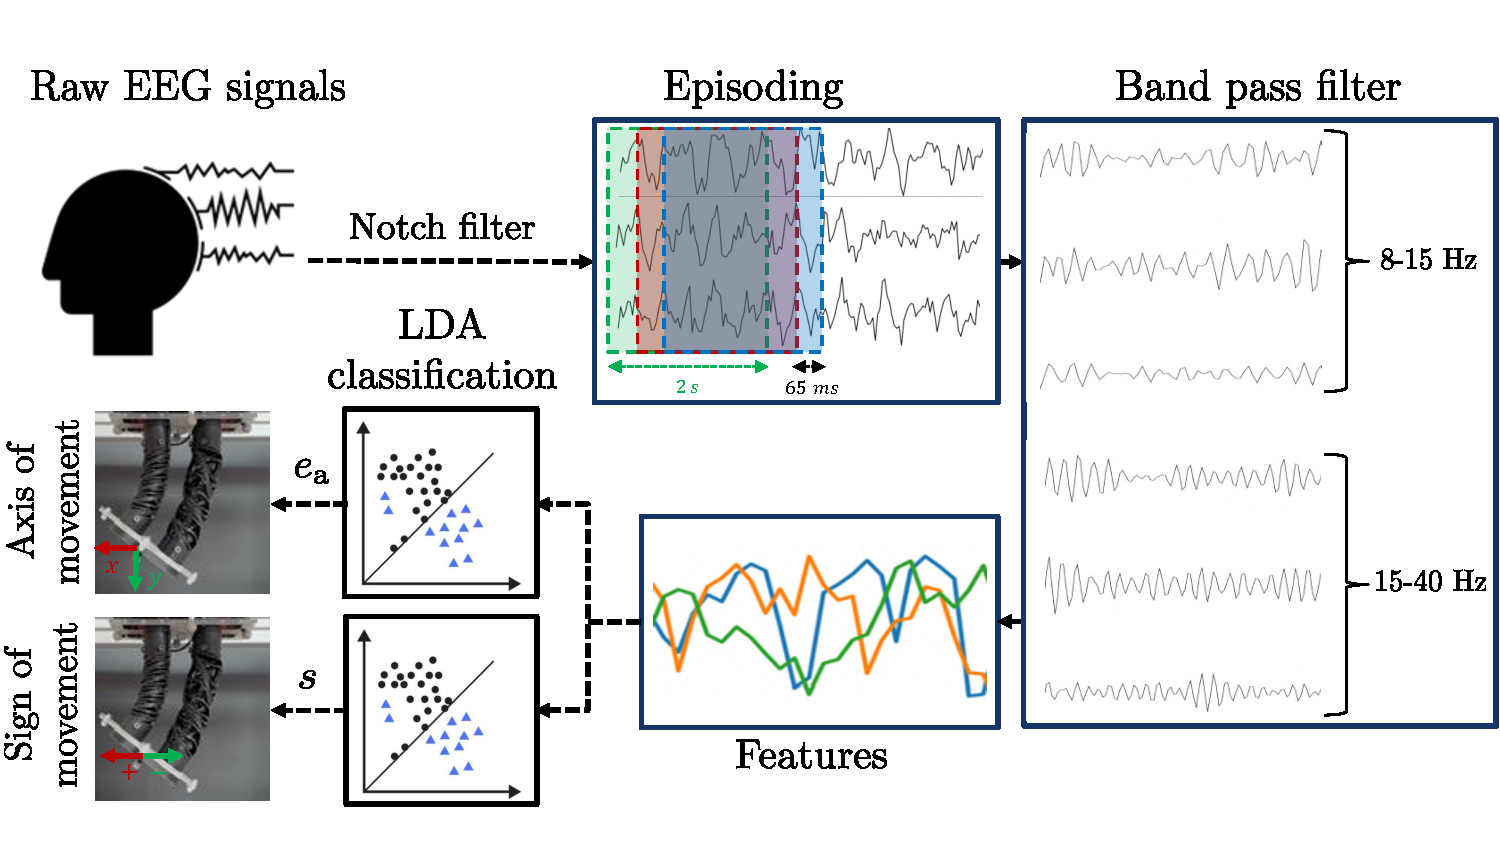
\includegraphics[width=\columnwidth]{braincontrol/figures/eeg_pipeline/eeg_pipeline_v3_compressed.pdf}
    \caption{EEG data processing pipeline: The EEG data is acquired in real-time, pre-processed, and divided into episodes and subbands. Next, we extract power features and pass them to two LDA classifiers: the first outputs the axis of movement (for example, moving along the x- or y-axis), and the second provides the sign of movement (for example, positive or negative movement along the active axis). These commands are then used to move the attractor in Cartesian space.}
    \label{fig:braincontrol:eeg_pipeline}
\end{center}
\end{figure}

\subsection{Background: modeling planar HSA robots}
Robots based on \glspl{HSA} rely on rods made of architected metamaterials to generate motion.  % ~\cite{truby2021recipe}
More specifically, twisting the rods along their handedness leads to an elongation of the rod~\cite{good2022expanding}. Combining multiple \glspl{HSA} in the setting of a parallel robot and actuating them with servo motors allows us to generate complex motion primitives and offer beneficial mechanical characteristics such as a high stiffness-to-weight ratio~\cite{stolzle2023modelling, good2022expanding}.

Prior work~\cite{stolzle2024experimental} has shown that the shape of planar \gls{HSA} robots can be approximated by one \gls{CS} segment. Therefore, we define the configuration of the system as $q = \begin{bmatrix}
    \kappa_\mathrm{be} & \sigma_\mathrm{sh} & \sigma_\mathrm{ax}
\end{bmatrix}^\mathrm{T} \in \mathbb{R}^3$.
We also have access to closed-form formulations of the forward kinematics $\pi: q \rightarrow \chi$ and inverse kinematics $\varrho: \chi \rightarrow q$ where $\chi = \begin{bmatrix}
    x^\mathrm{T} & \theta
\end{bmatrix}^\mathrm{T} \in SE(2)$ is the pose in task space and $\theta$ represents the end-effector orientation~\cite{stolzle2023experimental}.
We use the notation $J(q) = \frac{\partial x}{\partial q} \in \mathbb{R}^{2\times3}$ to refer to the kinematic Jacobian.

We can then derive the dynamics of the planar \gls{HSA} robot in Euler-Lagrangian form
\begin{equation}\label{eq:braincontrol:configuration_space_dynamics}
    M(q) \Ddot{q} + C(q,\dot{q})\dot{q} + G(q) + K \, (q-q^0) + D \, \dot{q} = \alpha(q,\phi),
\end{equation}
where $M(q), C(q,\dot{q}) \in \mathbb{R}^{3 \times 3}$ captures the inertial and Coriolis effects, $G(q) \in \mathbb{R}^3$ contributes the gravitational forces and $K \in \mathbb{R}^{3 \times 3}$ is the stiffness of the robot in its un-actuated state $q^0$. Furthermore, $D \in \mathbb{R}^{3 \times 3}$ is a positive-definite damping matrix. Finally, for the planar case, two \gls{HSA} rods are assumed to be actuated by the motor/twist angle $\phi \in \mathbb{R}^2$. As the handedness of the rods will be accounted for later, we state the actuation bounds as $0 \leq \phi_i \leq \phi_\mathrm{max} \: \forall i \in \{ 1, 2 \}$.
The auxetic trajectory~\cite{good2022expanding} causes the motors to act through the elasticity of the rods on the system and modify the axial rest length of the rod as a function of the twist strain~\cite{stolzle2023modelling}.
Furthermore, the stiffness of the rod can be modeled to be an affine function with respect to the twist strain~\cite{good2022expanding, stolzle2023modelling}. Both effects are captured in the actuation function $\alpha(q,\phi)$, which is nonlinear with respect to the actuation coordinate $\phi$ and affine in the configuration $q$.
%
Although this has never been done in the context of HSA robots, it is immediate to see that their dynamics \eqref{eq:braincontrol:configuration_space_dynamics} can be projected into operational space yielding the form~\cite{della2019exact, della2020model} % khatib1987unified
\begin{equation}\label{eq:braincontrol:operational_space_dynamics}
    \Lambda(q) \, \Ddot{x} + \mu(q,\dot{q}) \dot{q} + J_\mathrm{B}^{+\mathrm{T}} ( G(q) + K (q-q^0) + D \, \dot{q} ) = J_\mathrm{B}^{+\mathrm{T}} \alpha(q,\phi),
\end{equation}
where $J_\mathrm{B}^+(q) = B^{-1}J^\mathrm{T}(J B^{-1} J^\mathrm{T})^{-1} \in \mathbb{R}^{3\times2}$ is the dynamically consistent pseudo-inverse, $\Lambda(q) = (J \, B^{-1} J^\mathrm{T})^{-1} \in \mathbb{R}^{2 \times 2}$ is the inertia matrix in task space, and $\mu(q, \dot{q}) = \Lambda(q) \, (J B^{-1} C - \dot{J}) \in \mathbb{R}^{2 \times 3}$ collects the Cartesian Coriolis and centrifugal terms. % ~\cite{khatib1987unified}

\subsection{Cartesian impedance controller}\label{sub:braincontrol:computational_controller}
In previous work~\cite{stolzle2024experimental}, we have devised a model-based control strategy for regulating a planar \gls{HSA} robot towards a desired position in task space. %We propose here a new strategy that overcomes several limitations of that previous work which are critical for the application discussed in this paper - namely: (i) it involves a complex and computationally demanding planning procedure for identifying a suitable setpoint in configuration space, (ii) our configuration-space controller contains integral terms, making it unsafe for environment interactions, and (iii) it is based on a compensation of static forces in configuration-space thus not allowing us to shape the impedance characteristics in operational space.
%
We introduce below a novel control strategy that addresses some limitations of our previous work that are critical for the \gls{BMI} application. Namely, we (i) avoid computationally demanding planning procedures, (ii) remove integral terms that are unsafe for environment interaction, and (iii) enable impedance shaping in operational space. This Cartesian-space impedance controller is inspired by ~\cite{ott2008cartesian,della2020model}, but specifically designed for and tailored to \gls{HSA} robots. Crucially, we need to overcome the challenges of underactuation and the nonlinearity in the actuation - which were not present in that original work. %We, therefore, solve online a least-squares optimization problem, identifying the optimal actuation for generating the demanded task space forces.

\subsubsection{Proposed controller}
% We implement an operational space impedance action~\cite{ott2008cartesian, della2020model} that renders $x^\mathrm{at}$ an attractor of the closed-loop system.
We propose the following dynamic feedback law that renders $x^\mathrm{at}$ an attractor of the closed-loop system %~\cite{ott2008cartesian, della2020model} 
\begin{equation}\label{eq:braincontrol:cartesian_impedance_controller}
\begin{split}
    \tau =& \: J^\mathrm{T}(q) \, \left (K_x \, (x^\mathrm{at} - x) - D_x \, \dot{x} \right ) + G(q) + K \, (q-q^0)\\
    & \: + J^\mathrm{T}(q) \, J_\mathrm{B}^{+\mathrm{T}}(q) \, D \, \dot{q} + J^\mathrm{T}(q) \, \mu(q,\dot{q}) \left ( I_3 - J_\mathrm{B}^+(q) J(q) \right )\dot{q}
\end{split}
\end{equation}
where $\tau \in \mathbb{R}^3$ is the desired torque in configuration space, $G(q) + K \, (q-q^0)$ cancels the acting gravitational and elastic forces, and $J^\mathrm{T} J_\mathrm{B}^{+\mathrm{T}} D \, \dot{q}$ removes the natural dissipation in operational space.
We emphasize that because the system is underactuated, we need to cancel the stiffness directly in the configuration instead of operational space as done in previous work~\cite{della2020model}.
We can shape our desired impedance characteristics in Cartesian space with the PD term $f_\mathrm{PD} = K_x \, (x^\mathrm{at} - x) - D_x \, \dot{x} $ which is then projected into configuration space by premultiplying with $J^\mathrm{T}(q)$.

The term $\mu(q,\dot{q}) \left ( I_3 - J_\mathrm{B}^+(q) J(q) \right )\dot{q}$ decouples the operational space dynamics from the residual of the null-space dynamics~\cite{della2020model}\cite[Ch. 4]{ott2008cartesian}.
The identity $\dot{q} = J_\mathrm{B}^+ \, \dot{x} + Z^\mathrm{T} \, \nu_\mathrm{N}$, where $Z^\mathrm{T} \in \mathbb{R}^{3 \times 1}$ is the dynamically-consistent pseudo-inverse of the null space, allows us to formulate $\dot{q}$ as a sum of the task-space velocity $\dot{x}$ and the null-space velocity $\nu_\mathrm{N}$. Leveraging this identity, the Coriolis and centrifugal matrix $\mu(q,\dot{q})$ can be split into a term $\mu_x(q,\dot{q}) = \mu \, J_\mathrm{B}^+ \in \mathbb{R}^{2 \times 2}$ excited by $x$ and the expression $\mu_\mathrm{N}(q,\dot{q}) = \mu \, Z^\mathrm{T} \in \mathbb{R}^{2 \times 1}$ that is excited by the null-space coordinates resulting in $\mu(q,\dot{q}) \, \dot{q} = \mu_x(q,\dot{q}) \, \dot{x} + \mu_\mathrm{N}(q,\dot{q}) \, \nu_\mathrm{N}$.
This allows us to cancel the term $\mu_\mathrm{N}(q,\dot{q}) \, \nu_\mathrm{N}$ through $\mu(q,\dot{q}) \left ( I_3 - J_\mathrm{B}^+(q) J(q) \right )\dot{q}$ without having to compute the null space explicitly.


% The first step consists of establishing a PD feedback in Cartesian space
% \begin{equation}
%     f =  K_x \, (x^\mathrm{at} - x) - D_x \, \dot{x} + J_\mathrm{B}^{+\mathrm{T}} \, D \, \dot{q}. % + \eta(q, \dot{q}) J_\mathrm{B}^+ \left (G(q) + K \, q \right ).
% \end{equation}
% where $K_x \in \mathbb{R}^{2\times2}$ is the designed task-space stiffness and $D_x % \in \mathbb{R}^{2\times2}$ adds dissipation.
% We make use of the kinematic Jacobian to project the designed task-space force into % configuration space and additionally establish cancellation of the gravitational and % elastic forces with
% \begin{equation}
%     \tau = \alpha(q,\phi) = J^\mathrm{T}(q) \, f + G(q) + K \, (q-q^0).
% \end{equation}

In summary, the closed-loop dynamics in operational space can be stated as
\begin{equation}\label{eq:braincontrol:closed_loop_dynamics}
    \Lambda(q) \, \Ddot{x} + \mu(q,\dot{q}) \, J_\mathrm{B}^+ \, \dot{x} + K_x \, (x^\mathrm{at} - x) - D_x \, \dot{x} = 0,
\end{equation}
which results in $x^\mathrm{at}$ being the globally asymptotically stable equilibrium of the operational space dynamics.

% \begin{figure}
%     \centering
%     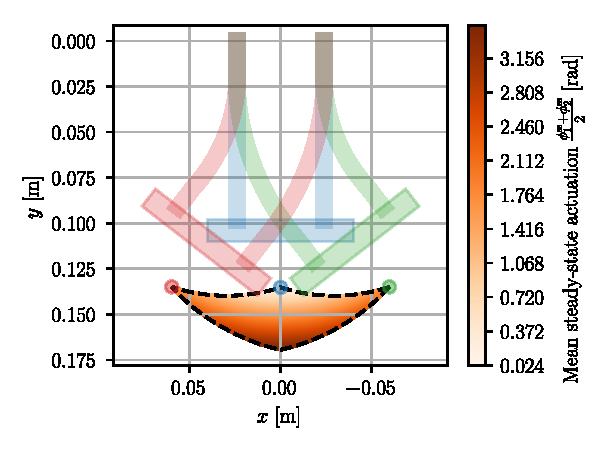
\includegraphics[width=0.85\columnwidth, trim={10 10 10 10}]{braincontrol/figures/workspace/operational_workspace_fpu_with_ee.pdf}
%     \caption{Operational workspace of a HSA robot with attached end-effector: the color displays the mean steady-state actuation $\frac{\phi_1^\mathrm{ss} + \phi_2^\mathrm{ss}}{2}$ necessary for the end-effector to remain at the position. Additionally, we visualize three example shapes: the straight configuration with $\phi^\mathrm{ss} = (0, 0)$ (blue), maximum clockwise bending with $\phi^\mathrm{ss} = (3.49, 0) \, \si{rad}$ (red), and maximum counter-clockwise bending with $\phi^\mathrm{ss} = (0, 3.49) \, \si{rad}$ (green).}
%     \label{fig:braincontrol:hsa_workspace}
% \end{figure}

\begin{figure*}
\begin{center}
    \subfigure[Operational workspace]{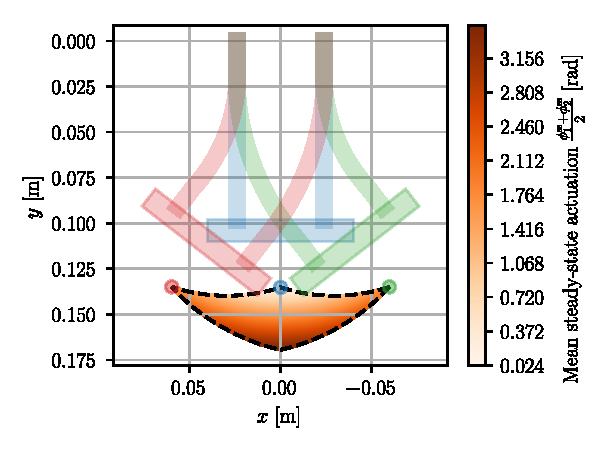
\includegraphics[width=0.36\linewidth]{braincontrol/figures/workspace/operational_workspace_fpu_with_ee.pdf}\label{fig:braincontrol:hsa_workspace}}
    \subfigure[Experimental setup]{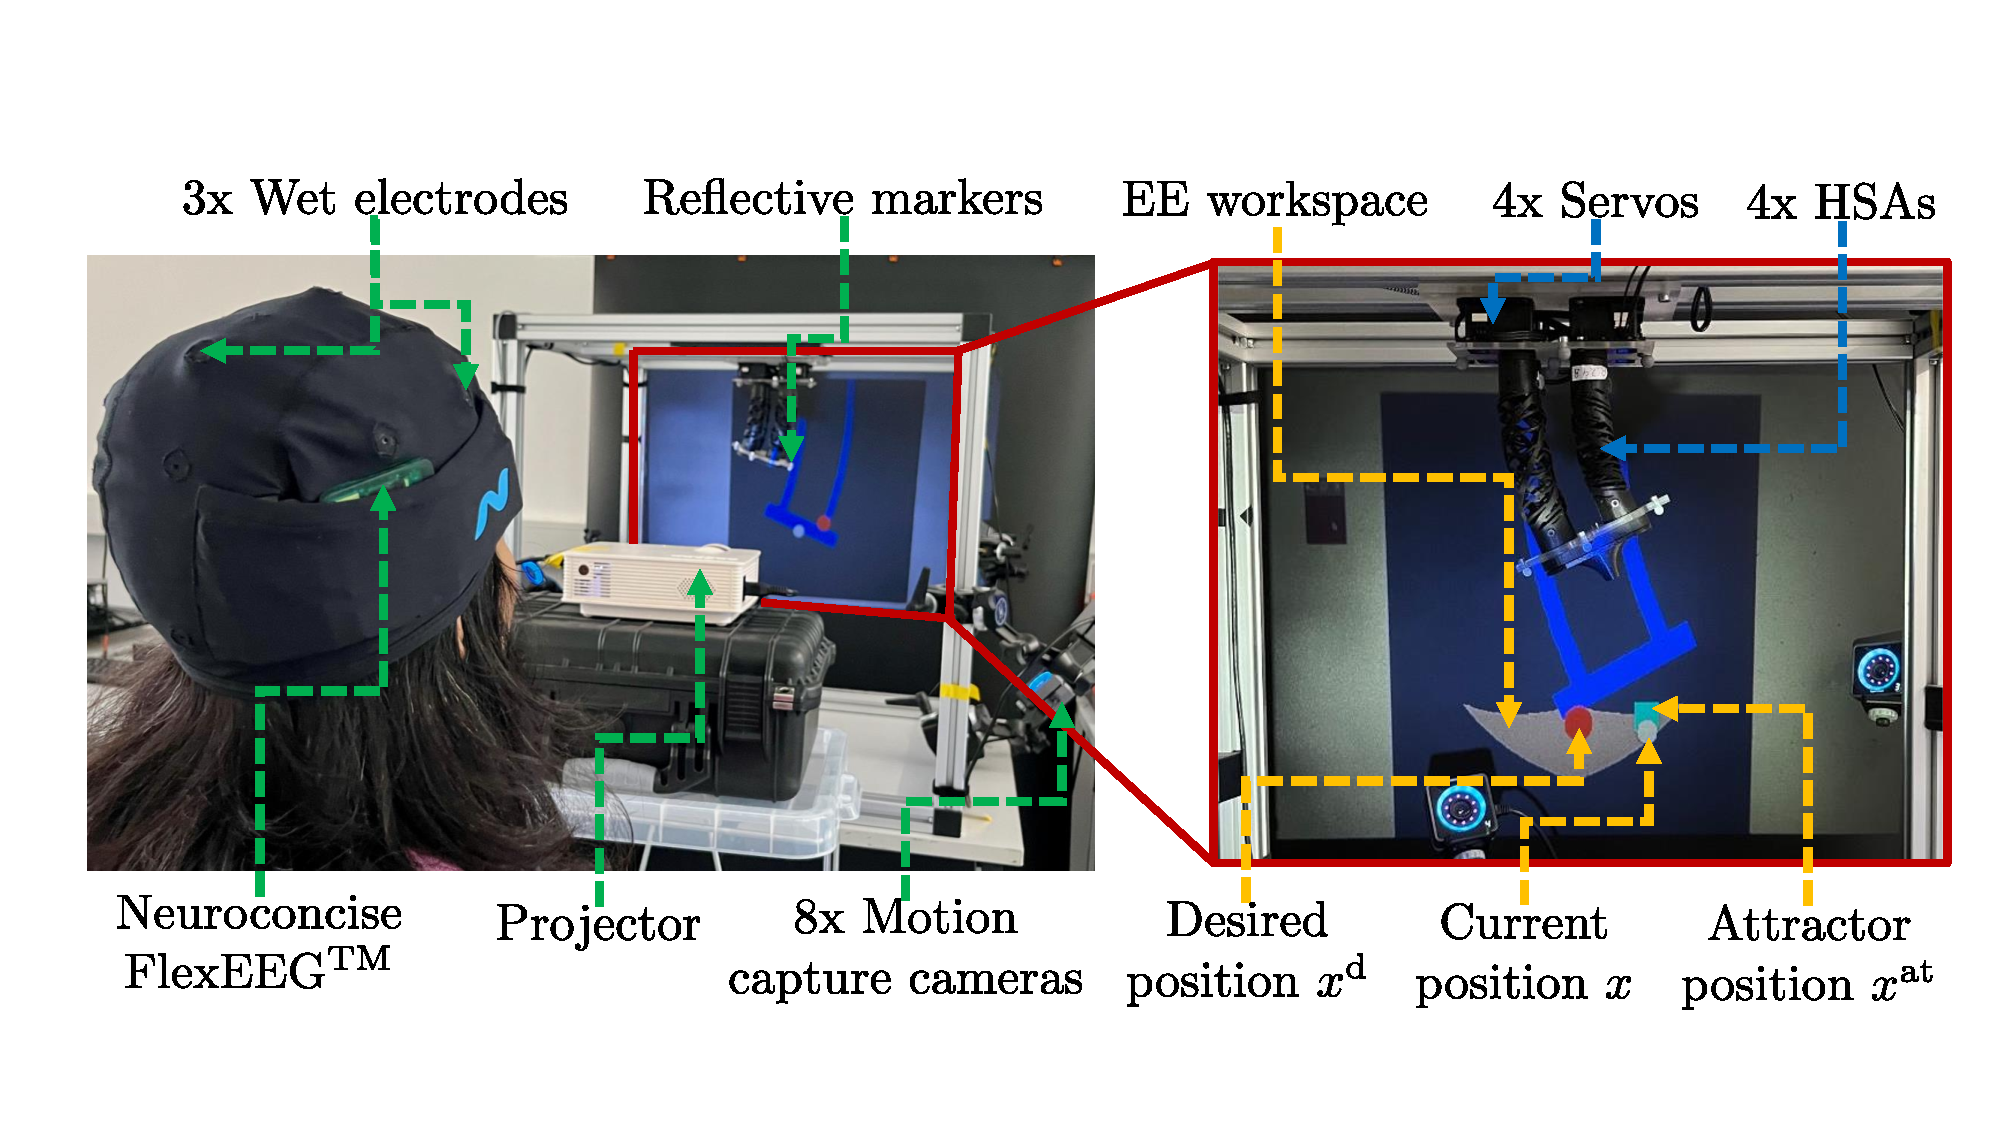
\includegraphics[width=0.63\linewidth]{braincontrol/figures/experimental_setup/experimental_setup_v3_cropped.pdf}\label{fig:braincontrol:experimental_setup}}
    \caption{\textbf{Panel (a:} Operational workspace of a HSA robot with attached end-effector: the color displays the mean steady-state actuation $\frac{\phi_1^\mathrm{ss} + \phi_2^\mathrm{ss}}{2}$ necessary for the end-effector to remain at the position. Additionally, we visualize three example shapes: the straight configuration with $\phi^\mathrm{ss} = (0, 0)$ (blue), maximum clockwise bending with $\phi^\mathrm{ss} = (3.49, 0) \, \si{rad}$ (red), and maximum counter-clockwise bending with $\phi^\mathrm{ss} = (0, 3.49) \, \si{rad}$ (green).
    \textbf{Panel (b):} The HSA robot is mounted platform-down to a motion capture cage with 8x Optitrack PrimeX 13 cameras, which track the 3D pose of the platform (i.e., the end-effector). A Dynamixel MX-28 servo actuates each of the four HSAs. We project a rendering of the current (white dot) and desired (red dot) end-effector position, the attractor (green square), and the operational workspace (grey area) onto the black screen in the background. The study subject wears a cap with the Neuroconcise FlexEEG sensor, and we acquire the data of three electrodes connected to the motor cortex.}
\end{center}
\end{figure*}

\begin{figure}
\begin{center}
    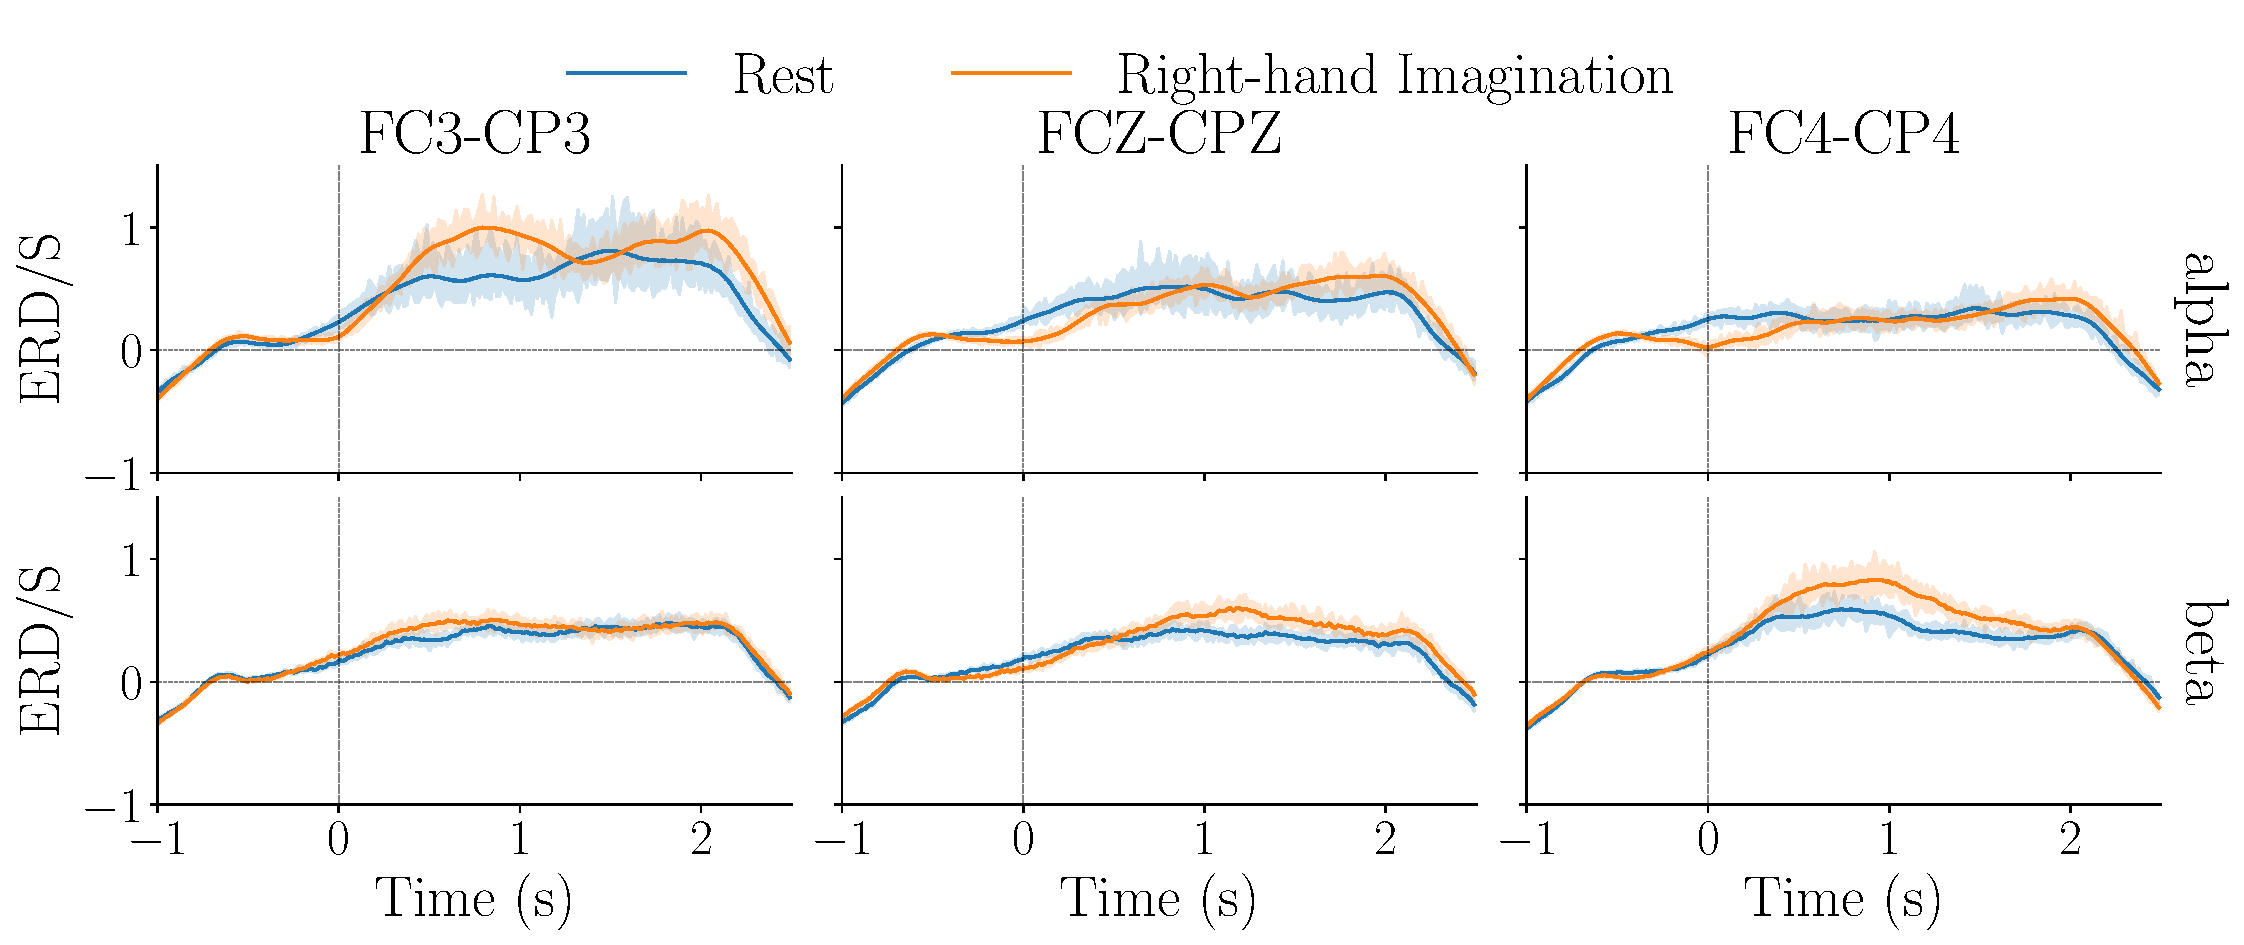
\includegraphics[width=0.85\columnwidth]{braincontrol/figures/eeg_pipeline/ERDS.pdf}
    \caption{ERD/S (overall average) over a time period of \SI{2.5}{s} of training data for right-hand Imagination v/s rest state including the Alpha and Beta bands of the EEG signals  where the cue is presented at \SI{0}{s}. We plot the data of three sensors (i.e., channels): FC3-CP3 (left), FCZ-CPZ (middle) and FC4-CP4 (right).}
    \label{fig:braincontrol:ERDS}
\end{center}
\end{figure}

\begin{figure*}[t]
    \centering
    \subfigure[End-effector x-coordinate]{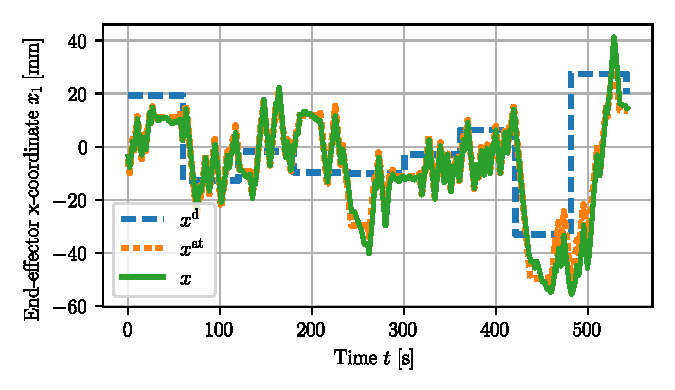
\includegraphics[width=0.47\textwidth, trim={5, 5, 5, 5}]{braincontrol/figures/setpoint_regulation/20231031_185546_pee_x.pdf}\label{fig:braincontrol:experimental_results:setpoint_regulation:brain:pee_x}}
    \subfigure[End-effector y-coordinate]{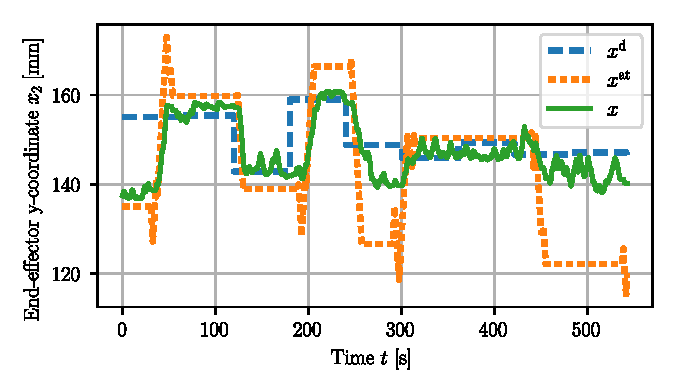
\includegraphics[width=0.47\textwidth, trim={5, 5, 5, 5}]{braincontrol/figures/setpoint_regulation/20231031_185546_pee_y.pdf}\label{fig:braincontrol:experimental_results:setpoint_regulation:brain:pee_y}}\\
    \subfigure[Configuration $q$]{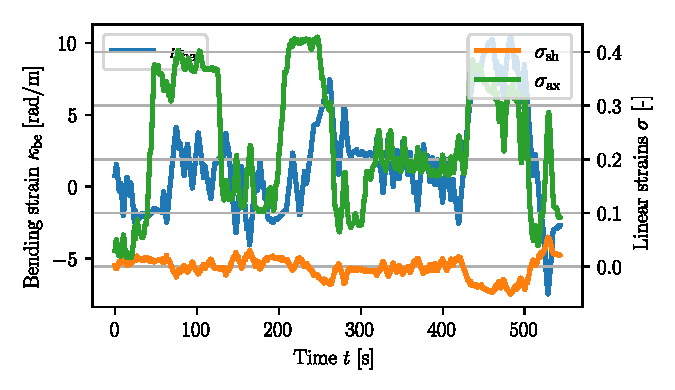
\includegraphics[width=0.47\textwidth, trim={5, 5, 5, 5}]{braincontrol/figures/setpoint_regulation/20231031_185546_q.pdf}\label{fig:braincontrol:experimental_results:setpoint_regulation:brain:q}}
    \subfigure[Control input $\phi$]{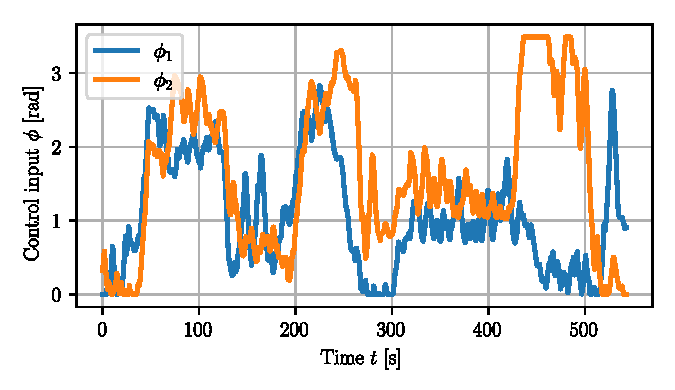
\includegraphics[width=0.47\textwidth, trim={5, 5, 5, 5}]{braincontrol/figures/setpoint_regulation/20231031_185546_phi.pdf}\label{fig:braincontrol:experimental_results:setpoint_regulation:brain:phi}}
    \caption{Experimental results for tracking a reference trajectory of nine step functions with motor imagery. \textbf{Panel (a) \& (b):} The x/y-coordinate of the end-effector position with the solid line denoting the actual position, the dotted line the attractor position, and the dashed line the reference (i.e., the setpoint).
    \textbf{Panel (c):} The evolution of the configuration.
    \textbf{Panel(d):} The saturated planar control inputs. }\label{fig:braincontrol:experimental_results:setpoint_regulation:brain}
\end{figure*}

\subsubsection{Mapping to Lagrangian forces}
%
Now that we have formulated our control law $\tau$ in configuration space, we need to identify a strategy to specify the motor angles $\phi \in \mathbb{R}^2$ such that $\alpha(q,\phi) \approx \tau$. Note that, in contrast to other continuum soft robots studied in literature~\cite{della2023model}, the actuation term $\alpha(q,\phi)$ is not affine in control. %, but rather a nonlinear function with respect to the actuation coordinates $\phi$. 
%Therefore, mapping configuration-space torques to motor commands is not straightforward.
In previous work~\cite{stolzle2023experimental}, we side-stepped this challenge by linearizing with respect to the steady-state actuation $\phi^\mathrm{ss}$: $A(q) = \lVert \frac{\partial \alpha}{\partial \phi}\rVert_{\phi=\phi^\mathrm{ss}}$ therefore recovering the usual scenario of an affine actuation function. Unfortunately, this is not possible in the setting of this work as i) we do not have access to such $\phi^\mathrm{ss}$, and ii) linearizing around $\phi$ causes the closed-loop system to become unstable. We, therefore, propose to formulate instead a nonlinear least-squares problem $\phi^\mathrm{d} = \argmin_\phi \frac{1}{2} \lVert \tau - \alpha(q,\phi) \rVert^2$ and solve it in real-time with a Levenberg Marquardt solver implemented in JAX~\cite{jaxopt_implicit_diff}.

We note that this approach is not guaranteed to be valid for the general case of an underactuated soft robot but for this particular structure of $\alpha(q,\phi) \in \mathbb{R}^3$ with $\phi \in \mathbb{R}^2$ it is possible to identify solutions $\phi$ with the Euclidean norm of the residual being smaller than $0.001$.
The source code of the controller is available on GitHub\footnote{\url{https://github.com/tud-phi/hsa-planar-control}}.
% Next, the actuation vector is linearized with respect to the current twist angle $A_\phi(q) = \frac{\partial \alpha}{\partial \phi} \big|_{\phi} \in \mathbb{R}^{3 \times 2}$. With that, we now have
% \begin{equation}
%     J^\mathrm{T} f = \alpha(q,\phi) + A_\phi(q) \, u
% \end{equation}